Chcemy w kwantowym czasie wielomianowym, czyli w \( \bigO(\log^k(A)) \) klasycznych obliczeniach i używając \( \bigO(\log^k(A)) \) bramek kwantowych znaleźć rząd elementu \( a \) modulo \( A \) z pewnym stałym prawdopodobieństem.
Określamy funkcję \( f : \set{0, 1, \ldots, N - 1} \to \natural \), gdzie \( N \) jest potęgą 2 przez:
\[
	f(x) = a^x \pmod{A}
\]
Funkcja \( f \) ma pewien okres \( r \) i jest różnowartościowa poza okresem (czyli \( f(x) = f(x + r) \) \\ i \( f(x) \neq f(x + r') \), jeśli \( r \nmid r' \)).
Równoważne sformułowanie zadania to wyznaczyć \( r \).

\textbf{Jak zakodować \( f \) w obwodzie?} \\
Konstruujemy bramkę \( O_f \), która ma \( n \) wejść i \( n \) wyjść, Bramka działa na \( n \) kubitach, które mogą mieć \( 2^n = N \) stanów podstawowych:
\[
	|\underbrace{00\ldots0}_n\rangle, |00\ldots1\rangle, \ldots, |11\ldots1\rangle
\]
Przekształcenie \( x \mapsto f(x) \pmod{A} \) niekoniecznie jest różnowartościowe, więc macierz która je opisuje nie jest unitarna ani odwracalna.
Podwajamy więc liczbę kubitów (\( 2n \) wejść i wyjść). Na weściu jest \( 2n \)-bitowy stan \( x \otimes y \), czyli sklejenie \( n \) bitów \( x \) i \( n \) bitów \( y \).
Wynikiem jest stan:
\[
	O_f(x \otimes y) = x \otimes (y \oplus f(x))
\]
Działanie jest odwracalne i ma przydatną własność:
\[
	O_f(x \otimes 0\ldots0) = x \otimes f(x)
\]

\newpage
Algorytm wygląda następująco:
\begin{greyframe}
	\begin{enumerate}
		\item Przygotuj \( 2n \) kubitów w stanie \( |0^n\rangle \otimes |0^n\rangle \).
		\item Nałóż na pierwsze \( n \) kubitów bramkę Hadamarda:
		      \[
			      |0^n\rangle \otimes |0^n\rangle \rightarrow \frac{1}{\sqrt{2^n}} \sum_{x=0}^{N-1} |x\rangle \otimes |0^n\rangle.
		      \]
		\item Nałóż na całość bramkę \( O_f \):
		      \[
			      \frac{1}{\sqrt{2^n}} \sum_{x=0}^{N-1} |x\rangle \otimes |0^n\rangle \rightarrow \frac{1}{\sqrt{2^n}} \sum_{x=0}^{N-1} |x\rangle \otimes f(x).
		      \]
		\item Zmierz ostatnie \( n \) kubitów.
		\item Nałóż na pierwsze \( n \) kubitów bramkę \( Q \).
		\item Zmierz pierwsze \( n \) kubitów -- wynik to \( j \cdot d \), czyli przypadkowa wielokrotność \( d \).
		      \begin{figure}[H]
			      \centering
			      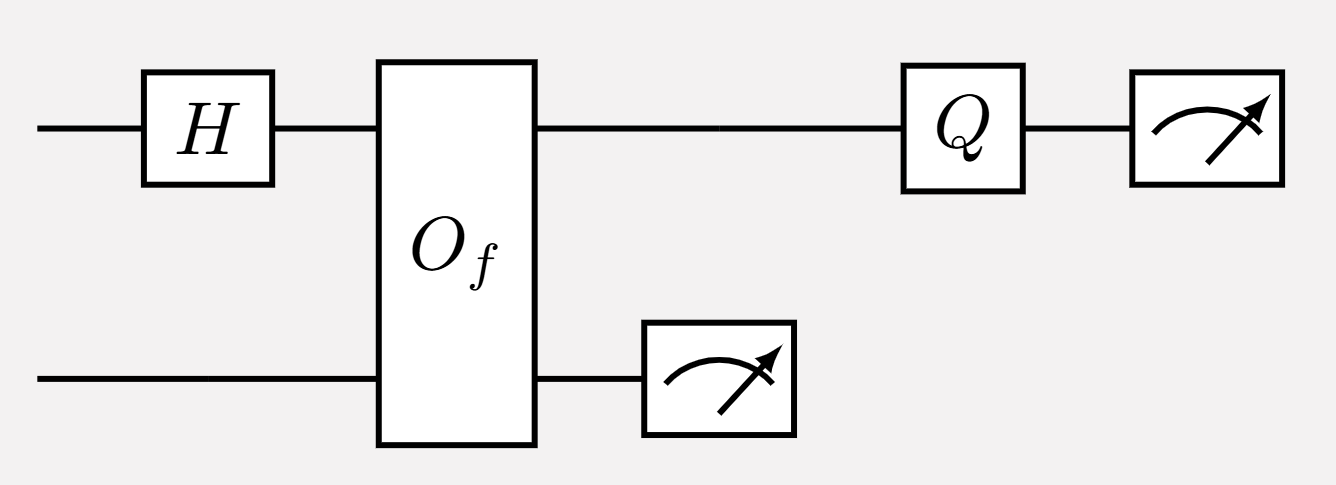
\includegraphics[width=0.5\textwidth]{img/shor_circuit.png}
		      \end{figure}
	\end{enumerate}
\end{greyframe}
Po kroku 4. na pierwszych \( n \) kubitach zostają tylko takie układy \( x \), dla których \( f(x) = y \) i~każdy z nich jest równie prawdopodobny.
Oznaczmy je przez
\[
	T = \set{x : 0 \leq x \leq N-1,\ f(x) = y}
\]
Na ostatnich \( n \) kubitach wykonujemy pomiar, otrzymując jakieś \( y \) i dalej te kubity nie są już potrzebne. Stan całego układu to:
\[
	\frac{1}{\sqrt{\abs{T}}} \sum_{x \in T} x \otimes y
\]
Załóżmy, że \( r \mid N \) i oznaczmy \( d = \frac{N}{r} \). Ze specyfiki funkcji \( f \) wynika, że istnieje takie \( s < r \), że \( T = \set{s, s + r, s + 2r, \ldots} \). Zatem \( \abs{T} = d \), czyli:
\[
	T = \set{s, s + r, s + 2r, \ldots, s + (d - 1)r}
\]
Na koniec, mając kubit w stanie
\[
	\frac{1}{\sqrt{d}} \sum_{x=0}^{N-1} b_x |x\rangle,
\]
gdzie \( b_x = \mathbbm{1}[x = s \!\!\pmod{r}] \), chcemy wyznaczyć \( r \) kwantową transformatą Fouriera.

\subsection*{Kwantowa transformata Fouriera}
Transformata Fouriera przekształca wektor \( v \) w wektor \( Q \cdot v \), gdzie \( Q \) jest macierzą Vandermonde'a:
\[
	Q = \frac{1}{\sqrt{N}} \begin{bmatrix}
		1      & 1            & 1               & \ldots & 1                   \\
		1      & \omega       & \omega^2        & \ldots & \omega^{N-1}        \\
		1      & \omega^2     & \omega^4        & \ldots & \omega^{2(N-1)}     \\
		1      & \omega^3     & \omega^6        & \ldots & \omega^{3(N-1)}     \\
		\vdots & \vdots       & \vdots          & \ddots & \vdots              \\
		1      & \omega^{N-1} & \omega^{2(N-1)} & \ldots & \omega^{(N-1)(N-1)}
	\end{bmatrix}
\]
Przeskalowanie przez \( \frac{1}{\sqrt{N}} \) jest potrzebne, żeby odwrotna transformata była taka sama czyli \\ \( Q \cdot \overline{Q^T} = I \).

Jako że \( Q \) jest unitarna, to możemy skonstruować bramkę Fouriera o \( n \) wejściach i \( n \) wyjściach, która mnoży \( n \) kubitów przez \( Q \).
Używamy do tego \( O(n^2) \) bramek \( H \) i \( R(\varphi) =
\brackets{\begin{smallmatrix}
		1 & 0 \\
		0 & e^{i\varphi}
	\end{smallmatrix}}
\).

Po przepuszczeniu kubitu
\[
	v = \frac{1}{\sqrt{d}} \sum_{x=0}^{N-1} b_x |x\rangle,
\]
przez bramkę \( Q \) otrzymujemy \( Q \cdot v = w = (w_1, \ldots, w_n) \), gdzie:
\[
	w_j = b_0 + b_1 \omega^j + b_2 \omega^{2j} + \ldots + b_{N-1} \omega^{(N-1)j},
\]
czyli, korzystając z tego, że \( b_x = \mathbbm{1}[x = s \!\!\pmod{r}] \), otrzymujemy:
\[
	w_j = \frac{1}{\sqrt{d}} \cdot \pars{ \omega^{s j} + \omega^{(s + r) j} + \ldots + \omega^{(s + (d - 1)r) j} } = \frac{1}{\sqrt{d}} \omega^{s j} \sum_{i = 0}^{d - 1} \omega^{i r j}.
\]
Jeśli \( N \mid r \cdot j \), to \( \omega^{r j} = 1 \), zatem
\[
	w_j = \sqrt{d} \cdot \omega^{s}
\]
Jeśli \( N \nmid r \cdot j \), to
\[
	w_j = \frac{1}{\sqrt{d}} \omega^{s} \cdot \frac{\omega^{r j d} - 1}{\omega^{r j} - 1} = \frac{1}{\sqrt{d}} \omega^{s} \cdot \frac{\omega^{j N} - 1}{\omega^{r j} - 1} = 0,
\]
Ponieważ \( N \mid r \cdot j \) wtedy i tylko wtedy, gdy \( d \mid j \), to wynikowym stanem jest:
\[
	\sqrt{d} \cdot \omega^s \cdot \sum_{d \mid x} |x\rangle
\]
A zatem kwantowa transformata Fouriera wykrywa okresowość.
Kubity w stanach: \[ s, s + r, s + 2r, \ldots \] po przejściu przez bramkę \( Q \) mogą mieć tylko stany: \[ d, 2d, 3d, \ldots, \] a przesunięcie \( s \) znika.

Mierząc taki kubit, dostajemy z równym prawdopodobieństem dowolny stan \( x \) taki, że \( d \mid x \). Na podstawie przypadkowego \( d = \frac{N}{r} \), chcemy poznać \( d \).
Powtarzamy więc cały algorytm kilkukrotnie -- za każdym razem dostajemy jakąś wielokrotność \( d \) (okres \( r \) jest taki sam, \( s \) może być inne).
Obliczając ich NWD, z dużym prawdopodobieństwem otrzymujemy \( d \).

W przypadku, kiedy \( r \nmid N \), po transformacie Fouriera i pomiarze możemy dostać każdy możliwy wynik. Jednak najbardziej prawdopodobne są te bliskie \( \frac{jN}{r} \) dla pewnego \( j \).
Ponieważ \( r \leq A \), to jeśli \( N > A^2 \), mając kilka pomiarów, też możemy odtworzyć \( r \).